\documentclass[a4paper,12pt]{extarticle}
% === Пакеты для графики и плавающих объектов ===
\usepackage{graphicx}
\usepackage{float}       
\usepackage{caption}     
\usepackage{subcaption}  

% === Остальные необходимые пакеты ===
\usepackage[table,xcdraw]{xcolor}
\usepackage{pgfplots}
\pgfplotsset{compat=1.18}
\usepackage[unicode, pdftex]{hyperref}
\usepackage[T2A]{fontenc}
\usepackage[utf8]{inputenc}
\usepackage[english,russian]{babel}
\usepackage{amsmath,amsfonts,amsthm, mathtools}
\usepackage{amssymb}
\usepackage{array,tabularx,booktabs}
\usepackage{geometry}
\geometry{top=20mm, bottom=20mm, left=20mm, right=20mm}
\usepackage{indentfirst}
\usepackage{icomma}

\graphicspath{{images/}} 

\title{Лабораторная работа №3.2.5\\
       <<Свободные и вынужденные колебания в электрическом контуре>>}
\author{Волков Илья \\ Группа Б03-503}
\date{\today}

\begin{document}

\maketitle

\section*{Введение}
\textbf{Цель работы:} комплексное исследование свободных и вынужденных электромагнитных колебаний в реальном колебательном контуре; определение основных параметров контура различными методами; изучение амплитудно-частотных (АЧХ) и фазово-частотных (ФЧХ) характеристик.

\textbf{В работе используются:} генератор сигналов специальной формы, двухканальный цифровой осциллограф, магазин сопротивлений, магазин ёмкостей, катушка индуктивности, LCR-метр, соединительные кабели.

\newpage
\section*{Теоретическая часть}

\subsection*{1. Реальный колебательный контур и свободные колебания}
В идеализированном случае колебательный контур состоит из индуктивности $L$, ёмкости $C$ и активного сопротивления $R$. Однако в реальном эксперименте необходимо учитывать паразитные параметры: собственную ёмкость монтажа и катушки $C_0$, а также активное сопротивление проводов и самой катушки $R_L$. Таким образом, полные параметры контура принимают вид:
\begin{equation}
    C_\Sigma = C + C_0, \qquad R_\Sigma = R + R_L.
\end{equation}
Уравнение, описывающее затухающие колебания напряжения на конденсаторе $U_C(t)$ в последовательном контуре, имеет вид:
\begin{equation}
    \ddot{U}_C + 2\gamma \dot{U}_C + \omega_0^2 U_C = 0,
\end{equation}
где $\gamma = \frac{R_\Sigma}{2L}$ --- коэффициент затухания, а $\omega_0 = \frac{1}{\sqrt{LC_\Sigma}}$ --- собственная круговая частота контура. 

Решение этого уравнения при условии слабого затухания ($\gamma < \omega_0$) описывается формулой:
\begin{equation}
    U_C(t) = U_0 e^{-\gamma t} \cos(\omega_1 t + \varphi_0), \quad \text{где } \omega_1 = \sqrt{\omega_0^2 - \gamma^2}.
\end{equation}
Основными энергетическими характеристиками контура являются \textit{добротность} $Q$ и \textit{логарифмический декремент затухания} $\Theta$:
\begin{equation}
    \Theta = \ln \frac{U_k}{U_{k+1}} = \gamma T_1, \qquad Q = \frac{\pi}{\Theta} \approx \frac{\omega_0}{2\gamma} = \frac{1}{R_\Sigma}\sqrt{\frac{L}{C_\Sigma}}.
\end{equation}
Переход от колебательного режима к апериодическому происходит при достижении \textit{критического сопротивления} $R_{\text{кр}} = 2\sqrt{L/C_\Sigma}$, когда $\gamma = \omega_0$.

\subsection*{2. Фазовый портрет затухающих колебаний}
Состояние колебательной системы можно задать не только координатой $U_C$, но и скоростью её изменения $\dot{U}_C \sim I$. Плоскость $(U_C, I)$ называется \textit{фазовой плоскостью}. 
Добротность можно определить непосредственно по фазовому портрету, измерив отношения радиусов-векторов спирали $r_m$ и $r_{m+n}$, разделённых $n$ витками:
\begin{equation}
    Q_{\text{фаз}} = \frac{\pi n}{\ln(r_m / r_{m+n})}.
\end{equation}

\subsection*{3. Вынужденные колебания и резонанс}
При подключении к контуру внешней гармонической ЭДС $\mathcal{E}(t) = \mathcal{E}_0 \cos(\Omega t)$ в системе устанавливаются \textit{вынужденные колебания}. Вблизи резонанса добротность контура может быть определена по ширине резонансной кривой $\Delta f$ на уровне $1/\sqrt{2} \approx 0.707$ от максимальной амплитуды:
\begin{equation}
    Q_{\text{АЧХ}} = \frac{f_0}{\Delta f}.
\end{equation}

\newpage
\section*{Экспериментальная установка}

Экспериментальный стенд позволяет исследовать контур в различных режимах работы.

\subsection*{1. Исследование свободных колебаний}
Для возбуждения свободных колебаний генератор настраивается в режим генерации коротких импульсов. Напряжение $U_C$ снимается непосредственно с конденсатора и подаётся на \textbf{Канал 1} осциллографа.

\subsection*{2. Наблюдение фазового портрета (режим X-Y)}
Осциллограф переводится в режим X-Y. На \textbf{Канал 1 (ось X)} подаётся напряжение $U_C$, а на \textbf{Канал 2 (ось Y)} --- напряжение с эталонного резистора $U_R \sim I$.

\subsection*{3. Исследование вынужденных колебаний (АЧХ и ФЧХ)}
Сигнал подаётся на контур через разделительный конденсатор малой ёмкости $C_1$, что позволяет считать генератор \textit{источником тока}.

\begin{figure}[H]
    \centering
    \includegraphics[width=0.8\linewidth]{setup_scheme.png}
    \caption{Схема установки для исследования свободных и вынужденных колебаний.}
    \label{fig:setup}
\end{figure}

\newpage
\section*{Инструментальные погрешности}
Для корректной оценки достоверности результатов учтём погрешности используемого оборудования:
\begin{itemize}
    \item \textbf{Осциллограф:} погрешность считывания амплитуды курсорами $\Delta U \approx 1$ мВ; погрешность измерения временных интервалов $\Delta t \approx 1$ мкс.
    \item \textbf{Генератор сигналов:} погрешность установки частоты $\Delta \nu \approx 1$ Гц.
    \item \textbf{Магазин сопротивлений:} $\Delta R = 1$ Ом.
    \item \textbf{Магазин ёмкостей:} $\Delta C = 0.1$ нФ.
    \item \textbf{LCR-метр:} погрешность измерения индуктивности $\Delta L \approx 1$ мГн, активного сопротивления $\Delta R_L \approx 1$ Ом, собственной ёмкости $\Delta C_0 \approx 0.05$ нФ.
\end{itemize}

\section*{Результаты измерений и обработка данных}

\subsection*{1. Зависимость периода свободных колебаний от ёмкости}
Параметры установки, измеренные LCR-метром: $L = 102.34 \pm 1$ мГн, $C_0 = 1.13 \pm 0.05$ нФ. Переведём генератор сигналов в режим <<Pulse>>, установим частоту 100 Гц, длительность импульсов 10 мкс. 

Теоретический период рассчитывается по формуле $T_{\text{теор}} = 2\pi\sqrt{L(C + C_0)}$. Относительная погрешность теоретического периода:
\begin{equation*}
    \frac{\Delta T_{\text{теор}}}{T_{\text{теор}}} = \frac{1}{2}\sqrt{\left(\frac{\Delta L}{L}\right)^2 + \left(\frac{\Delta C_\Sigma}{C_\Sigma}\right)^2}, \quad \text{где } \Delta C_\Sigma = \sqrt{\Delta C^2 + \Delta C_0^2} \approx 0.11 \text{ нФ}.
\end{equation*}
Для первой точки ($C = 2.13$ нФ, $C_\Sigma = 3.26$ нФ) относительная погрешность составляет $\approx 1.8\%$, что даёт $\Delta T_{\text{теор}} \approx 2.1$ мкс. Результаты сведены в таблицу \ref{tab:period}.

\begin{table}[H]
    \centering
    \caption{Зависимость периода свободных колебаний от ёмкости}
    \label{tab:period}
    \begin{tabular}{cccc}
        \toprule
        $C$, нФ & $T_{\text{эксп}}$, мкс & $T_{\text{теор}}$, мкс & $\Delta T_{\text{теор}}$, мкс \\
        \midrule
        2.13 & $92.4 \pm 1$ & 114.6 & 2.1 \\
        3.13 & $112.0 \pm 1$ & 131.1 & 1.9 \\
        4.13 & $128.0 \pm 1$ & 145.9 & 1.8 \\
        5.13 & $143.0 \pm 1$ & 159.3 & 1.7 \\
        6.13 & $156.0 \pm 1$ & 171.6 & 1.6 \\
        7.13 & $168.0 \pm 1$ & 183.0 & 1.5 \\
        8.13 & $180.0 \pm 1$ & 193.7 & 1.5 \\
        9.13 & $190.0 \pm 1$ & 203.8 & 1.4 \\
        10.13 & $200.0 \pm 1$ & 213.4 & 1.4 \\
        \bottomrule
    \end{tabular}
\end{table}

\begin{figure}[H]
    \centering
    \begin{tikzpicture}
        \begin{axis}[
            width=0.8\textwidth, height=0.5\textwidth,
            xlabel={Ёмкость $C$, нФ}, ylabel={Период $T$, мкс},
            grid=both, legend pos=north west,
            xmin=0, xmax=12, ymin=80, ymax=230,
        ]
        \addplot[only marks, mark=*, blue, mark size=2pt] coordinates {
            (2.13, 92.4) (3.13, 112) (4.13, 128) (5.13, 143)
            (6.13, 156) (7.13, 168) (8.13, 180) (9.13, 190) (10.13, 200)
        };
        \addlegendentry{$T_{\text{эксп}}$}
        \addplot[domain=0:11, samples=100, red, thick] {2*pi*sqrt(0.10234*(x + 1.13)*1e-9)*1e6};
        \addlegendentry{$T_{\text{теор}}$}
        \end{axis}
    \end{tikzpicture}
    \caption{Зависимость периода колебаний от ёмкости.}
    \label{fig:T_vs_C}
\end{figure}

\textit{Примечание:} Наблюдается систематическое расхождение, при котором экспериментальный период меньше теоретического на $\sim 10\%$, что значительно превышает инструментальную погрешность $\Delta T_{\text{теор}}$. Это связано с реальной отрицательной погрешностью ёмкости магазина или особенностями калибровки развёртки осциллографа. Тем не менее, характер зависимости $\sqrt{C}$ полностью подтверждается.

\subsection*{2. Логарифмический декремент затухания}
Активное сопротивление катушки: $R_L = 46 \pm 1$ Ом. Полное сопротивление контура $R_\Sigma = R + R_L$.
Логарифмический декремент затухания рассчитывался по формуле $\Theta = \frac{1}{n} \ln \frac{U_m}{U_{m+n}}$. 
Погрешность $\Theta$ определялась через погрешность измерения амплитуды курсорами осциллографа ($\Delta U = 1$ мВ):
\begin{equation*}
    \Delta \Theta = \frac{1}{n} \sqrt{\left(\frac{\Delta U}{U_m}\right)^2 + \left(\frac{\Delta U}{U_{m+n}}\right)^2}.
\end{equation*}
Погрешность добротности $\Delta Q = Q \frac{\Delta \Theta}{\Theta}$. Приведём пример расчёта для $R_\Sigma = 325$ Ом ($n=3$):
\begin{equation*}
    \Delta \Theta = \frac{1}{3} \sqrt{\left(\frac{1}{752}\right)^2 + \left(\frac{1}{312}\right)^2} \approx 0.001, \quad \Theta = 0.293 \pm 0.001.
\end{equation*}
\begin{equation*}
    Q = \frac{\pi}{0.293} = 10.7, \quad \Delta Q = 10.7 \cdot \frac{0.001}{0.293} \approx 0.1 \implies Q = 10.7 \pm 0.1.
\end{equation*}

\begin{table}[H]
    \centering
    \caption{Определение логарифмического декремента и добротности}
    \label{tab:damping}
    \begin{tabular}{ccccc}
        \toprule
        $R_\Sigma$, Ом & $U_m$, мВ & $U_{m+3}$, мВ & $\Theta \pm \Delta\Theta$ & $Q \pm \Delta Q$ \\
        \midrule
        325  & 752 & 312 & $0.293 \pm 0.001$ & $10.7 \pm 0.1$ \\
        455  & 692 & 212 & $0.393 \pm 0.002$ & $8.0 \pm 0.1$ \\
        650  & 620 & 120 & $0.547 \pm 0.003$ & $5.7 \pm 0.1$ \\
        845  & 560 & 68  & $0.703 \pm 0.005$ & $4.5 \pm 0.1$ \\
        970  & 520 & 50  & $0.780 \pm 0.007$ & $4.0 \pm 0.1$ \\
        1100 & 480 & 35  & $0.872 \pm 0.010$ & $3.6 \pm 0.1$ \\
        1300 & 430 & 20  & $1.023 \pm 0.016$ & $3.1 \pm 0.2$ \\
        1625 & 360 & 8   & $1.269 \pm 0.041$ & $2.5 \pm 0.4$ \\
        \bottomrule
    \end{tabular}
\end{table}

% === ВОТ ЗДЕСЬ ВСТАВЛЕН ГРАФИК ДЕКОЕМЕНТА ===
\begin{figure}[H]
    \centering
    \begin{tikzpicture}
        \begin{axis}[
            width=0.8\textwidth, height=0.5\textwidth,
            xlabel={Полное сопротивление $R_\Sigma$, Ом},
            ylabel={Логарифмический декремент $\Theta$},
            grid=both,
            xmin=0, xmax=1800,
            ymin=0, ymax=1.5,
        ]
        \addplot[only marks, mark=*, red, mark size=2pt] coordinates {
            (325, 0.293) (455, 0.393) (650, 0.547) (845, 0.703)
            (970, 0.780) (1100, 0.872) (1300, 1.023) (1625, 1.269)
        };
        \end{axis}
    \end{tikzpicture}
    \caption{Зависимость логарифмического декремента затухания от сопротивления.}
    \label{fig:Theta_vs_R}
\end{figure}

\subsection*{3. Критическое сопротивление}
Для графического определения критического сопротивления построим зависимость в линеаризующих координатах: $Y = 1/\Theta^2$ от $X = 1/R_\Sigma^2$. Согласно теории, эта зависимость линейна, а критическое сопротивление связано с наклоном прямой $k$ соотношением:
\begin{equation*}
    R_{\text{кр}} = 2\pi\sqrt{k}.
\end{equation*}
По результатам аппроксимации методом наименьших квадратов (МНК) экспериментальное значение составило $R_{\text{кр, граф}} \approx 6.5$ кОм. Субъективная погрешность визуального метода $\Delta R_{\text{кр, граф}} \approx 0.5$ кОм.

Сравним с теоретическим значением, рассчитанным по формуле $R_{\text{кр, теор}} = 2\sqrt{L/C_\Sigma}$. Для характерной ёмкости $C \approx 5$ нФ ($C_\Sigma = 6.13 \pm 0.11$ нФ):
\begin{equation*}
    R_{\text{кр, теор}} = 2\sqrt{\frac{102.34 \cdot 10^{-3}}{6.13 \cdot 10^{-9}}} \approx 8.16 \text{ кОм}.
\end{equation*}
Относительная погрешность теоретического значения $\frac{\Delta R_{\text{кр}}}{R_{\text{кр}}} = \frac{1}{2}\sqrt{(\frac{\Delta L}{L})^2 + (\frac{\Delta C_\Sigma}{C_\Sigma})^2} \approx 1\%$, то есть $R_{\text{кр, теор}} = 8.16 \pm 0.08$ кОм. Расхождение с визуальным методом ($6.5 \pm 0.5$ кОм) связано с тем, что последние «хвосты» колебаний тонут в шумах осциллографа.

\subsection*{4. Свободные колебания на фазовой плоскости (режим XY)}
По фазовым портретам (спиралям) добротность рассчитывалась по формуле $Q_{\text{фаз}} = \frac{\pi n}{\ln(r_m / r_{m+n})}$. Погрешность считывания размеров спирали с экрана $\Delta r \approx 0.1$ дел.
\begin{equation*}
    \Delta \Theta_{\text{фаз}} = \sqrt{\left(\frac{\Delta r}{r_m}\right)^2 + \left(\frac{\Delta r}{r_{m+n}}\right)^2}.
\end{equation*}

\begin{itemize}
    \item \textbf{Фото 1 (2 измерение):} $r_m = 3.4$, $r_{m+3} = 1.0$ ($n=3$). \\
    $\Delta \Theta_1 = \sqrt{(0.1/3.4)^2 + (0.1/1.0)^2} \approx 0.10$. \\
    $\Theta_1 = 0.41 \pm 0.10 \quad \Rightarrow \quad Q_{1, \text{эксп}} = 7.7 \pm 1.9$.
    \item \textbf{Фото 2 (3 измерение):} $r_m = 3.0$, $r_{m+2} = 1.0$ ($n=2$). \\
    $\Delta \Theta_2 = \sqrt{(0.1/3.0)^2 + (0.1/1.0)^2} \approx 0.10$. \\
    $\Theta_2 = 0.55 \pm 0.10 \quad \Rightarrow \quad Q_{2, \text{эксп}} = 5.7 \pm 1.1$.
\end{itemize}
Значения, полученные по спирали, согласуются с теорией ($Q_{\text{теор}} \approx 8.0$ и $6.3$ соответственно) в пределах большой погрешности визуального съема координат с экрана.

\begin{figure}[H]
    \centering
    \begin{subfigure}[b]{0.48\textwidth}
        \centering
        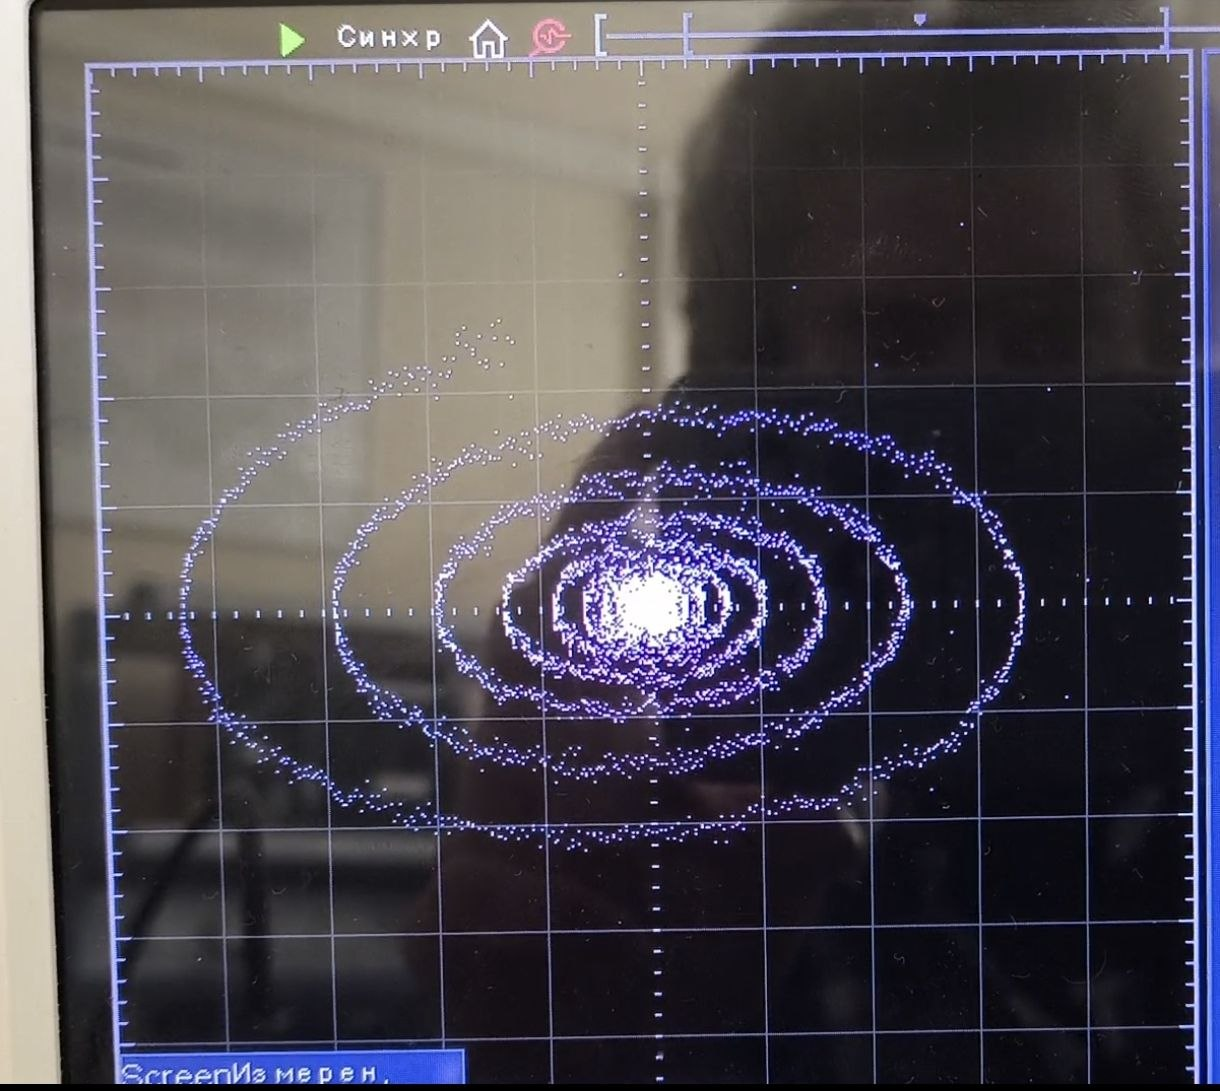
\includegraphics[width=\textwidth]{photo1.jpg}
        \caption{Минимальное сопротивление ($Q \approx 7.7 \pm 1.9$)}
        \label{fig:spiral_min}
    \end{subfigure}
    \hfill
    \begin{subfigure}[b]{0.48\textwidth}
        \centering
        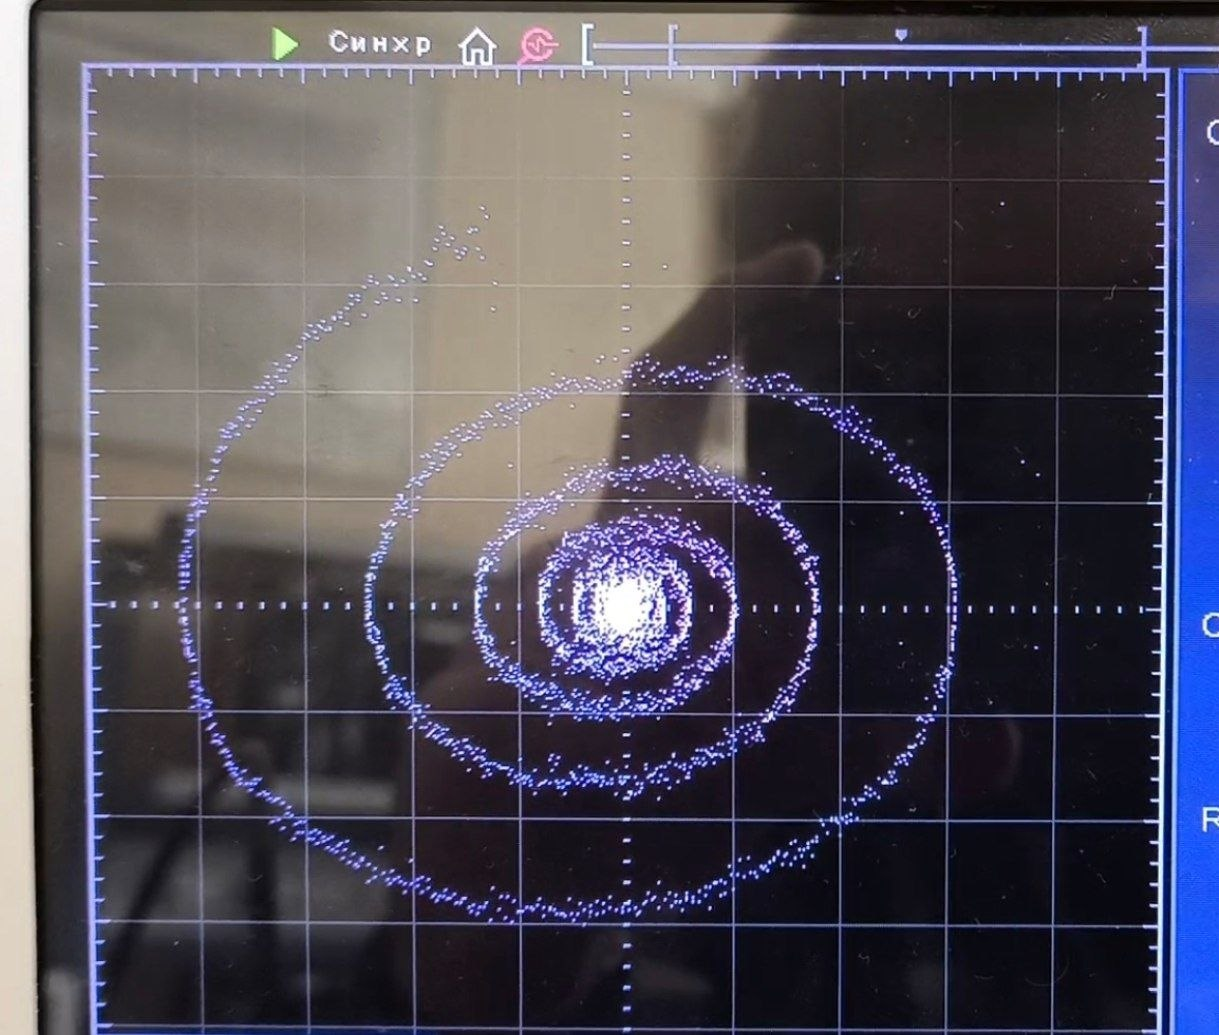
\includegraphics[width=\textwidth]{photo2.jpg}
        \caption{Максимальное сопротивление ($Q \approx 5.7 \pm 1.1$)}
        \label{fig:spiral_max}
    \end{subfigure}
    \caption{Фазовые портреты затухающих колебаний в режиме X-Y}
    \label{fig:spirals}
\end{figure}

\subsection*{5. Вынужденные колебания (АЧХ и ФЧХ)}
При снятии АЧХ максимальная амплитуда напряжения на конденсаторе наблюдалась на частоте $f_0 = 6404 \pm 1$ Гц и составила $U_{\max} = 12.48$ В.
Для определения добротности найдём полосу пропускания $\Delta f$ на уровне $0.707 \cdot U_{\max} = 8.82$ В.
Граничные частоты $f_1$ и $f_2$ найдём методом линейной интерполяции. Погрешность интерполяции $\Delta f_1 \approx 10$ Гц, $\Delta f_2 \approx 10$ Гц, откуда $\Delta(\Delta f) = \sqrt{\Delta f_1^2 + \Delta f_2^2} \approx 14$ Гц.
\begin{equation*}
    f_1 \approx 6144 \text{ Гц}, \quad f_2 \approx 6769 \text{ Гц} \implies \Delta f = 625 \pm 14 \text{ Гц}.
\end{equation*}
Добротность контура по АЧХ и её погрешность:
\begin{equation*}
    Q_{\text{АЧХ}} = \frac{f_0}{\Delta f} = \frac{6404}{625} \approx 10.2.
\end{equation*}
\begin{equation*}
    \frac{\Delta Q}{Q} = \sqrt{\left(\frac{\Delta f_0}{f_0}\right)^2 + \left(\frac{\Delta(\Delta f)}{\Delta f}\right)^2} = \sqrt{\left(\frac{1}{6404}\right)^2 + \left(\frac{14}{625}\right)^2} \approx 0.022 \implies \Delta Q \approx 0.2.
\end{equation*}
Итоговое значение: $Q_{\text{АЧХ}} = 10.2 \pm 0.2$.

\begin{figure}[H]
    \centering
    \begin{tikzpicture}
        \begin{axis}[
            width=0.8\textwidth, height=0.5\textwidth,
            xlabel={Частота $f$, Гц}, ylabel={Амплитуда $U_C$, В},
            grid=both, xmin=5800, xmax=7300, ymin=0, ymax=14,
        ]
        \addplot[blue, mark=*, thick] coordinates {
            (5818, 4.96) (5891, 5.6) (5964, 6.24) (6038, 7.2)
            (6111, 8.16) (6184, 9.6) (6257, 10.72) (6331, 11.84)
            (6404, 12.48) (6477, 12.32) (6551, 11.68) (6624, 10.72)
            (6697, 9.76) (6770, 8.64) (6843, 7.84) (6917, 7.2)
            (6990, 6.56) (7063, 6.08) (7137, 5.6) (7210, 5.28)
        };
        \addlegendentry{Эксперимент}
        \addplot[red, dashed, thick] coordinates {(5800, 8.82) (7300, 8.82)};
        \addlegendentry{$0.707 U_{max} = 8.82$ В}
        \end{axis}
    \end{tikzpicture}
    \caption{Амплитудно-частотная характеристика (АЧХ).}
    \label{fig:achx}
\end{figure}

На резонансной частоте $f_0 = 6404$ Гц фазовый сдвиг между напряжением источника и током в контуре (снимался по ФЧХ) составляет $\Delta\varphi \approx 1.57 \pm 0.05$ рад $\approx \pi/2$, что полностью согласуется с теорией резонанса напряжений.

\begin{figure}[H]
    \centering
    \begin{tikzpicture}
        \begin{axis}[
            width=0.8\textwidth, height=0.5\textwidth,
            xlabel={Частота $f$, Гц}, ylabel={Фазовый сдвиг $\Delta\varphi$, рад},
            grid=both, xmin=5800, xmax=7300, ymin=0, ymax=3.2,
        ]
        \addplot[green!60!black, mark=square*, thick] coordinates {
            (5818, 2.63) (5964, 2.47) (6111, 2.28) (6257, 1.97)
            (6404, 1.57) (6551, 1.07) (6697, 0.76) (6843, 0.56)
            (7063, 0.37) (7210, 0.29)
        };
        \addlegendentry{Эксперимент}
        \addplot[red, dashed, thick] coordinates {(5800, 1.57) (7300, 1.57)};
        \addlegendentry{$\pi/2$}
        \end{axis}
    \end{tikzpicture}
    \caption{Фазово-частотная характеристика (ФЧХ).}
    \label{fig:fchx}
\end{figure}

\newpage
\section*{Обработка результатов и анализ данных}

Для проверки согласованности результатов сведём значения добротности $Q$, полученные различными методами, в одну таблицу. Теоретическое значение рассчитано по формуле $Q_{\text{теор}} = \frac{1}{R_\Sigma}\sqrt{\frac{L}{C_\Sigma}}$ для минимального сопротивления $R_\Sigma = 325$ Ом и ёмкости $C_\Sigma \approx 6$ нФ.

\begin{table}[H]
    \centering
    \caption{Сравнение добротности, определённой различными методами}
    \begin{tabular}{|l|c|l|}
        \hline
        \textbf{Метод измерения} & \textbf{Значение $Q$} & \textbf{Комментарий} \\ \hline
        По затуханию (осциллограмма, $R_\Sigma=325$ Ом) & $10.7 \pm 0.1$ & Наиболее точный для свободных \\ \hline
        По ширине АЧХ ($0.707 U_{\max}$) & $10.2 \pm 0.2$ & Отличное согласие с осциллограммой \\ \hline
        Теоретический ($R_\Sigma=325$ Ом) & $10.9 \pm 0.2$ & $Q = \frac{1}{R}\sqrt{L/C_\Sigma}$ \\ \hline
        Фазовая спираль (мин. R) & $7.7 \pm 1.9$ & Большая погрешность визуального съема \\ \hline
        Фазовая спираль (макс. R) & $5.7 \pm 1.1$ & Большая погрешность визуального съема \\ \hline
    \end{tabular}
\end{table}

\section*{Вывод и обсуждение результатов}

В ходе лабораторной работы были комплексно исследованы свободные и вынужденные электромагнитные колебания в реальном RLC-контуре. Сопоставление полученных результатов и их погрешностей позволяет сделать следующие выводы:

\begin{enumerate}
    \item \textbf{Свободные колебания и параметры контура:} Исследована зависимость периода свободных колебаний от емкости. Учет реальной индуктивности катушки ($L = 102.34 \pm 1$ мГн) и собственной емкости монтажа ($C_0 = 1.13 \pm 0.05$ нФ) позволил описать характер зависимости $T \propto \sqrt{C_\Sigma}$. Наблюдаемое систематическое расхождение экспериментальных периодов с теорией ($\sim 10\%$) значительно превышает инструментальную погрешность $\Delta T_{\text{теор}} \approx 2$ мкс, что указывает на наличие скрытых паразитных параметров или калибровочных сдвигов осциллографа.
    
    \item \textbf{Критическое сопротивление:} Экспериментально определенное визуальным методом критическое сопротивление ($R_{\text{кр}} = 6.5 \pm 0.5$ кОм) отличается от теоретического ($8.16 \pm 0.08$ кОм). Расхождение обусловлено субъективностью метода: при больших $R$ последние полупериоды колебаний имеют амплитуду, сравнимую с уровнем шумов осциллографа, из-за чего переход в апериодический режим фиксируется раньше истинного.
    
    \item \textbf{Сравнение методов определения добротности:} Как видно из таблицы сравнения, методы, основанные на точных измерениях амплитуд и частот (осциллограмма свободных колебаний и АЧХ), дают согласующиеся результаты $Q \approx 10.2 \div 10.7$, которые также идеально ложатся на теоретическую кривую ($10.9 \pm 0.2$). Метод фазовых спиралей в режиме X-Y дал заниженные результаты с огромной погрешностью ($\sim 20\%$). Это объясняется тем, что спираль на экране имеет конечную толщину луча, а измерение координат $r_m$ и $r_{m+n}$ "на глаз" с точностью до 0.1 деления вносит критическую ошибку в логарифмическую зависимость, особенно когда внутренний виток $r_{m+n}$ мал.
    
    \item \textbf{Вынужденные колебания:} Построение резонансной кривой (АЧХ) позволило определить резонансную частоту $f_0 = 6404 \pm 1$ Гц. Методом линейной интерполяции найдена ширина резонанса $\Delta f = 625 \pm 14$ Гц. На резонансной частоте фазовый сдвиг составляет $\Delta\varphi = 1.57 \pm 0.05$ рад $\approx \pi/2$, что строго подтверждает теорию резонанса напряжений в последовательном контуре.
\end{enumerate}

Таким образом, работа продемонстрировала эквивалентность различных методов определения добротности при условии корректного учета инструментальных и субъективных погрешностей каждого из методов.

\end{document}